\section{Периодические решения и предельные циклы}
\begin{definition}{Периодическое решение}{periodic_sol}
	Решение $x=x(t)$, $y=y(t)$ автономной системы:
	\begin{equation} \label{eq:284}
		\begin{cases}
			\dv{x}{t} = f(x,y) \\
			\dv{y}{t} = g(x,y)
		\end{cases} \quad (284)
	\end{equation}
	называется \textbf{периодическим}, если существует $T > 0$ такое, что для любого $t$ выполнено $\begin{cases} x(t+T) = x(t) \\ y(t+T) = y(t) \end{cases}$. Во избежание вырожденных случаев мы подразумеваем, что $x(t)$ и $y(t)$ не являются постоянными функциями.
\end{definition}

\begin{itemize}
	\item Периодическое решение имеет траекторию (орбиту), которая представляет собой замкнутую кривую, проходящую снова и снова при изменении $t$. Мы будем называть такую орбиту циклом.
\end{itemize}

Есть ли в системе \eqref{eq:284} циклы? \\
Мы предполагаем, что ф-ции $f(x,y)$ и $g(x,y)$ определены и непрерывно дифференцируемы в каждой точке плоскости $xOy$.

\begin{example}
	(задача 218) \\
	$\begin{cases} \dv{x}{t} = -y \\ \dv{y}{t} = x \end{cases}$ \qquad Решение: $\begin{cases} y = A\cos t + B\sin t \\ x = -A\sin t + B\cos t \end{cases} \quad (286)$ \\
	Значения $x,y$ повторяются через $2\pi$, что означает замкнутость орбиты.
\end{example}

Обобщим этот результат. \\
В любой двумерной линейной системе $X' = AX$, где собственными значениями матрицы $A$ является пара чисто мнимых чисел $\pm i\beta$, $\beta \neq 0$, все постоянные орбиты являются циклами (точнее, эллипсами).

\begin{itemize}
	\item \textbf{Система Лотки-Вольтерры} — системы хищник-жертва имеет орбиты в первом квадранте, которые являются циклами, окружающими точку равновесия $\qty(\frac{d}{c}, \frac{a}{b})$.
	\begin{equation} \label{eq:287}
		\begin{cases}
			\dv{x}{t} = ax - bxy \\
			\dv{y}{t} = -dy + cxy
		\end{cases} \quad (287)
	\end{equation}
	где $x$ — кол-во жертв, $y$ — кол-во хищников, $t$ — время. $a,b,c,d > 0$, $a,b,c,d = \text{const}$, отраж. взаимодействия между видами.
	
	\item При формулировке ур-ний Вольтерра использовали предположения:
	\begin{enumerate}
		\item[(1)] В отсутствие хищников популяция жертв будет расти (в краткосрочной перспективе).
		\item[(2)] При отсутствии добычи популяция хищников будет экспоненциально сокращаться.
	\end{enumerate}
	$\hookrightarrow$ мальтузианская модель.
	
	\item У системы Лотки-Вольтерра \eqref{eq:287} есть 2 точки покоя. Найдем их, приравняв к нулю $\dv{x}{t}, \dv{y}{t}$:
	\begin{equation} \label{eq:288}
		\begin{cases}
			ax - bxy = 0 \\
			-dy + cxy = 0
		\end{cases} \iff
		\begin{cases}
			x(a - by) = 0 \\
			y(-d + cx) = 0
		\end{cases} \iff
		\begin{bmatrix}
			\begin{cases} x = 0 \\ y = 0 \end{cases} \\
			\begin{cases} x = \frac{d}{c} \\ y = \frac{a}{b} \end{cases}
		\end{bmatrix} \quad (288)
	\end{equation}
\end{itemize}

Точка $(0,0)$: отсутствуют хищники и жертвы (интереса не представляет). \\
В окрестности точки $\qty(\frac{d}{c}, \frac{a}{b})$, проведем линеаризацию системы \eqref{eq:287} в виде:
$\begin{cases} x = \frac{d}{c} + \tilde{x} \\ y = \frac{a}{b} + \tilde{y} \end{cases}$, где $\tilde{x}, \tilde{y}$ — малые добавки.

Подставим $x,y$ в \eqref{eq:287}:
\begin{align*}
	\begin{cases}
		\dv{\tilde{x}}{t} &= a\qty(\frac{d}{c} + \tilde{x}) - b\qty(\frac{d}{c} + \tilde{x})\qty(\frac{a}{b} + \tilde{y}) = \cancel{\frac{ad}{c}} + a\tilde{x} - \cancel{\frac{da}{c}} - \frac{bd}{c}\tilde{y} - b\tilde{x}\tilde{y} \\
		\dv{\tilde{y}}{t} &= -d\qty(\frac{a}{b} + \tilde{y}) + c\qty(\frac{d}{c} + \tilde{x})\qty(\frac{a}{b} + \tilde{y}) = -\cancel{\frac{ad}{b}} - d\tilde{y} + \cancel{\frac{ad}{b}} + \frac{ac}{b}\tilde{x} + c\tilde{x}\tilde{y}
	\end{cases}
\end{align*}

Отбросим нелинейные члены $\tilde{x}\tilde{y}$, получим линеаризованную систему:
\begin{equation} \label{eq:289}
	\begin{cases}
		\dv{\tilde{x}}{t} = -\frac{bd}{c}\tilde{y} \\
		\dv{\tilde{y}}{t} = \frac{ac}{b}\tilde{x}
	\end{cases} \quad (289) \iff
	\begin{cases}
		dt = -\frac{d\tilde{x}}{\frac{bd}{c}\tilde{y}} \\
		dt = \frac{d\tilde{y}}{\frac{ac}{b}\tilde{x}}
	\end{cases} \implies
	-\frac{d\tilde{x}}{\frac{bd}{c}\tilde{y}} = \frac{d\tilde{y}}{\frac{ac}{b}\tilde{x}} \iff
	\frac{ac}{b}\tilde{x} d\tilde{x} = -\frac{bd}{c}\tilde{y} d\tilde{y}
\end{equation}
Проинтегрируем обе части ур-ния: $\frac{ac}{2b}\tilde{x}^2 = -\frac{bd}{2c}\tilde{y}^2 + C_1$, $C_1 > 0$, $\tilde{x} = x - \frac{d}{c}, \tilde{y} = y - \frac{a}{b}$ \\
т.е. траектория (орбита) представляет собой эллипс с центром в точке $\qty(\frac{d}{c}, \frac{a}{b})$:
\begin{equation} \label{eq:290}
	\frac{ac}{2b}\qty(x - \frac{d}{c})^2 + \frac{bd}{2c}\qty(y - \frac{a}{b})^2 = C_1 \quad (290)
\end{equation}

\noindent
\begin{minipage}{0.48\textwidth}
	\centering
	\begin{tikzpicture}[scale=0.9]
		\draw[-stealth] (0,0) -- (6,0) node[right] {время};
		\draw[-stealth] (0,-0.5) -- (0,3) node[above, align=center] {размер\\популяции};
		
		% Prey
		\draw[blue, thick, smooth, samples=100, domain=0:5.5] plot (\x, {1.5 + 0.8*sin(\x*100)});
		\node[blue] at (5.8, 2.3) {жертва};
		
		% Predator
		\draw[orange, thick, smooth, samples=100, domain=0:5.5] plot (\x, {1 + 0.5*sin(\x*100 - 90)});
		\node[orange, align=left] at (4, 1.8) {синусоидальная\\зависимость};
	\end{tikzpicture}
	\\ \small решения $x(t), y(t)$ линеариз. системы Лотки-Вольтерра
\end{minipage}
\hfill
\begin{minipage}{0.48\textwidth}
	\centering
	\begin{tikzpicture}[scale=0.9, decoration={markings, mark=at position 0.3 with {\arrow{stealth}}, mark=at position 0.8 with {\arrow{stealth}}}]
		\draw[-stealth] (-1,0) -- (5,0) node[right] {$x$};
		\draw[-stealth] (0,-1) -- (0,3.5) node[above] {$y$};
		
		\coordinate (Center) at (3,2);
		\filldraw (Center) circle (1.5pt);
		\draw[dashed] (Center) -- (3,0) node[below] {$\frac{d}{c}$};
		\draw[dashed] (Center) -- (0,2) node[left] {$\frac{a}{b}$};
		
		\draw[postaction={decorate}, blue, thick] (Center) ellipse (0.5 and 0.3);
		\draw[postaction={decorate}, blue, thick] (Center) ellipse (1.0 and 0.6);
		\draw[postaction={decorate}, blue, thick] (Center) ellipse (1.5 and 0.9);
	\end{tikzpicture}
\end{minipage}

\vspace{0.5cm}

\underline{\textbf{Пример 2:}} 
\begin{equation} \label{eq:291}
	\begin{cases}
		\dv{x}{t} = -y + x(1 - x^2 - y^2) \\
		\dv{y}{t} = x + y(1 - x^2 - y^2)
	\end{cases} \quad (291)
\end{equation}
Точка покоя $(0,0)$ — неустойчивый фокус. \\
Система имеет периодическое решение $x(t) = \cos t$, $y(t) = \sin t$ (единичная окружность $\Gamma$).

\noindent
\begin{minipage}{0.3\textwidth}
	\centering
	\begin{tikzpicture}[scale=1.2, decoration={markings, mark=at position 0.5 with {\arrow{stealth}}}]
		\draw[-stealth] (-1.5,0) -- (1.5,0) node[right] {$x$};
		\draw[-stealth] (0,-1.5) -- (0,1.5) node[above] {$y$};
		
		% Limit cycle
		\draw[blue, thick, postaction={decorate}] (0,0) circle (1);
		
		% Inner spiral
		\draw[blue, domain=0:6, samples=60, postaction={decorate}] plot ({0.1*exp(0.1*\x)*cos(\x r)}, {0.1*exp(0.1*\x)*sin(\x r)});
		
		% Outer spirals
		\draw[blue, domain=0:6, samples=60, postaction={decorate}] plot ({(1 + 0.5*exp(-0.5*\x))*cos(\x r + 2)}, {(1 + 0.5*exp(-0.5*\x))*sin(\x r + 2)});
		\draw[blue, domain=0:6, samples=60, postaction={decorate}] plot ({(1 + 0.5*exp(-0.5*\x))*cos(\x r - 2)}, {(1 + 0.5*exp(-0.5*\x))*sin(\x r - 2)});
	\end{tikzpicture}
\end{minipage}
\begin{minipage}{0.65\textwidth}
	Орбиты, начинающиеся внутри себя либо вне единичной окр-ти $\Gamma$, закручиваются по спирали по направлению к $\Gamma$ при $t \to \infty$. \\
	Можно назвать $\Gamma$ предельным циклом, т.к. к нему приближаются все близлежащие траектории при $t \to \infty$. \\
	Т.к. более того, $\Gamma$ является притягивающим предельным циклом. \\
	Предельные циклы могут быть отталкивающими, если близлежащие траектории приближаются к ним при $t \to -\infty$.
\end{minipage}

Циклы в системе Лотки-Вольтерры не являются предельными циклами, т.к. близлежащие траектории сами являются циклами и находятся на постоянном расстоянии от данного цикла.

\vspace{0.3cm}
\noindent\underline{\textbf{13.03}}
\section{Циклы и точки равновесия}

\begin{itemize}
	\item Циклы всегда должны окружать одну или несколько точек равновесия. \\
	Этот факт можно использовать, чтобы исключить наличие циклов.
\end{itemize}

\begin{example}
	Модель конкурирующих видов: \\
	$\begin{cases} \dv{x}{t} = x(2 - x - y) \\ \dv{y}{t} = y(1 - x - 4y) \end{cases}$ \\
	не может иметь циклов в биологически значимом I квадранте, поскольку его точки равновесия — это $(0,0), (0, 1/4), (2,0)$ и $(7/3, -1/3)$, ни одна из которых не находится в I квадранте. \\
	Первый квадрант — это пример односвязной области (<<область без дыр>>).
\end{example}

\begin{definition}{Односвязная область}{simply_connected}
	Область $\Omega$ односвязная, если любую простую (без самопересечений) кривую, лежащую в области $\Omega$, можно стянуть в точку, не выходя из $\Omega$.
\end{definition}

\vspace{0.5cm}
\begin{center}
	\begin{tikzpicture}[scale=1]
		% 1
		\begin{scope}[shift={(0,0)}]
			\draw[-stealth] (-2,0) -- (2,0);
			\draw[-stealth] (0,-2) -- (0,2);
			\node[above] at (0, 2.5) {1. односвязная область};
			\draw[thick, blue, pattern=north east lines, pattern color=blue!50] (0.5,0) to[out=90,in=0] (0.5,1.5) to[out=180,in=90] (-1,0.5) to[out=-90,in=180] (0,-1) to[out=0,in=-90] (0.5,0);
		\end{scope}
		
		% 2
		\begin{scope}[shift={(5,0)}]
			\draw[-stealth] (-2,0) -- (2,0);
			\draw[-stealth] (0,-2) -- (0,2);
			\node[above, align=center] at (0, 2.2) {2. неодносвязная \\ область};
			\draw[thick, blue, pattern=north east lines, pattern color=blue!50, even odd rule] (0,0) ellipse (1.5 and 1) (0,0) ellipse (0.7 and 0.4);
		\end{scope}
		
		% 3
		\begin{scope}[shift={(10,0)}]
			\draw[-stealth] (-2,0) -- (2,0);
			\draw[-stealth] (0,-1) -- (0,2);
			\node[above, align=center] at (0, 2.2) {3. односвязная \\ область};
			\draw[thick, blue, pattern=north east lines, pattern color=blue!50] (-1.5, 0.2) -- (1.5, 0.2) -- (1.5, 1.5) -- (-1.5, 1.5) -- cycle;
			\node at (0, 0.8) {\Large I};
		\end{scope}
	\end{tikzpicture}
\end{center}

\vspace{0.5cm}
\textcolor{orange}{Содержит ли область циклы?}

\begin{theorem}{Об отсутствии циклов в односвязной области}{no_cycles_simply_conn}
	Если область $\Omega$ односвязная и не содержит точек равновесия системы \eqref{eq:284}, то в $\Omega$ нет циклов.
\end{theorem}

\begin{theorem}{Теорема Пуанкаре-Бендиксона}{poincare_bendixson_1}
	позволяет выяснить существование циклов в области.
	Двусвязную (кольцевую) область между двумя простыми замкнутыми кривыми:
\end{theorem}

\begin{center}
	\begin{tikzpicture}
		\begin{scope}[shift={(0,0)}]
			\node at (0, 1.5) {1.};
			\draw[thick, blue] (0,0) circle (0.8);
			\node[align=center, font=\small] at (0, -1.2) {простая \\ замкнутая \\ кривая};
		\end{scope}
		
		\begin{scope}[shift={(3,0)}]
			\node at (0, 1.5) {2.};
			\draw[thick, blue] (-0.5, -0.5) .. controls (1, 1) and (-1, 1) .. (0.5, -0.5);
			\node[align=center, font=\small] at (0, -1.2) {не является ни \\ простой, ни \\ замкнутой};
		\end{scope}
		
		\begin{scope}[shift={(6,0)}]
			\node at (0, 1.5) {3.};
			\draw[thick, blue] (0,0) to[out=45, in=0] (0, 0.8) to[out=180, in=135] (0,0) to[out=-45, in=0] (0, -0.8) to[out=180, in=-135] (0,0);
			\node[align=center, font=\small] at (0, -1.2) {замкнутая \\ (непростая) \\ кривая};
		\end{scope}
		
		\begin{scope}[shift={(10, 0.5)}]
			\draw[thick, blue, pattern=north west lines, pattern color=blue!30, even odd rule] 
			(0,0) circle (1.5) 
			(-0.2, 0.1) circle (0.5);
			\node at (0, 0) {$C_{in}$};
			\node at (1.2, 1.2) {$C_{out}$};
		\end{scope}
	\end{tikzpicture}
\end{center}

\begin{theorem}{Теорема Пуанкаре-Бендиксона}{poincare_bendixson_2}
	Пусть $\Omega$ - область, состоящая из двух простых замкнутых кривых $C_{out}$ и $C_{in}$, где $C_{in}$ находится внутри $C_{out}$, и кольцевая область находится между ними. Предположим, что $\Omega$ не содержит точек равновесия системы
	\begin{equation} \label{eq:292}
		\begin{cases}
			\dv{x}{t} = f(x,y) \\
			\dv{y}{t} = g(x,y)
		\end{cases} \quad (292)
	\end{equation}
	где $f, g$ непрерывно дифференцируемы в $\mathbb{R}^2$. Предположим также, что существует траектория $(x(t), y(t))$, которая остается в $\Omega$ для всех $t \ge 0$. Тогда либо эта траектория сама является циклом в $\Omega$, либо она движется по спирали к некоторому предельному циклу в $\Omega$ при $t \to \infty$.
\end{theorem}

\begin{itemize}
	\item Заметим, что при выполнении условий $th_2$ область $\Omega$ обязана содержать цикл.
	\item \textbf{Следствие} (из th Пуанкаре-Бендиксона) \\
	Для того, чтобы доказать существование циклов, требуется найти кривые $C_{out}, C_{in}$ (а значит и область $\Omega$, располож. между ними), т.г. векторное поле $\qty(\dv{x}{t}, \dv{y}{t})$ для системы \eqref{eq:292} во всех точках кривых $C_{out}, C_{in}$ направлено внутрь области $\Omega$.
	Это гарантирует, что траектория, которая начинается в $\Omega$, останется в $\Omega$ при $t \ge 0$.
\end{itemize}

\begin{minipage}{0.3\textwidth}
	\centering
	\begin{tikzpicture}[scale=1]
		\draw[thick, blue, pattern=north west lines, pattern color=blue!30, even odd rule] 
		(0,0) circle (1.5) 
		(0,0) circle (0.6);
		
		\node at (-1.7, 1) {$C_{out}$};
		\node at (-0.3, -0.3) {$C_{in}$};
		\node at (1, 0) {$\Omega$};
		
		% Arrows pointing inwards from Cout
		\draw[-stealth, thick] (1.5, 0) -- (1.1, 0);
		\draw[-stealth, thick] (-1.5, 0) -- (-1.1, 0);
		\draw[-stealth, thick] (0, 1.5) -- (0, 1.1);
		\draw[-stealth, thick] (0, -1.5) -- (0, -1.1);
		
		% Arrows pointing outwards from Cin (into Omega)
		\draw[-stealth, thick] (0.6, 0) -- (0.9, 0);
		\draw[-stealth, thick] (-0.6, 0) -- (-0.9, 0);
		\draw[-stealth, thick] (0, 0.6) -- (0, 0.9);
		\draw[-stealth, thick] (0, -0.6) -- (0, -0.9);
	\end{tikzpicture}
\end{minipage}
\begin{minipage}{0.65\textwidth}
	векторное поле в граничных точках области $\Omega$
\end{minipage}

\vspace{0.5cm}
\begin{itemize}
	\item \underline{\textbf{Пример 1:}} система $\begin{cases} \dv{x}{t} = -y + x(1-x^2-y^2) \\ \dv{y}{t} = x + y(1-x^2-y^2) \end{cases}$ \\
	Уже рассматривали ранее (\eqref{eq:291} + фазовые траектории поиск).
\end{itemize}

\begin{minipage}{0.3\textwidth}
	\centering
	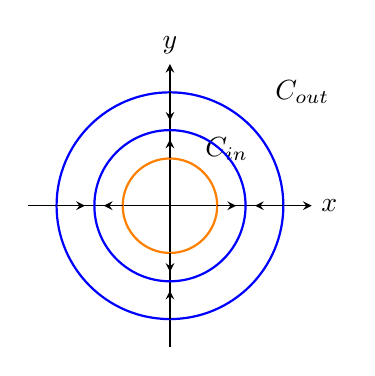
\begin{tikzpicture}[scale=1.2]
		\draw[-stealth] (-1.5,0) -- (1.5,0) node[right] {$x$};
		\draw[-stealth] (0,-1.5) -- (0,1.5) node[above] {$y$};
		
		\draw[thick, blue] (0,0) circle (1.2); \node at (1.4, 1.2) {$C_{out}$};
		\draw[thick, orange] (0,0) circle (0.5); \node at (0.6, 0.6) {$C_{in}$};
		
		\draw[blue, thick, -stealth] (0,0) circle (0.8);
		
		% Arrows Cout
		\draw[-stealth] (1.2, 0) -- (0.9, 0);
		\draw[-stealth] (0, 1.2) -- (0, 0.9);
		\draw[-stealth] (-1.2, 0) -- (-0.9, 0);
		\draw[-stealth] (0, -1.2) -- (0, -0.9);
		
		% Arrows Cin
		\draw[-stealth] (0.5, 0) -- (0.7, 0);
		\draw[-stealth] (0, 0.5) -- (0, 0.7);
		\draw[-stealth] (-0.5, 0) -- (-0.7, 0);
		\draw[-stealth] (0, -0.5) -- (0, -0.7);
	\end{tikzpicture}
\end{minipage}
\begin{minipage}{0.65\textwidth}
	Мы хотим использовать th Пуанкаре-Бендиксона, чтобы показать, что эта система имеет цикл, который должен заключать в себе единственную точку равновесия $(0,0)$. \\
	Для этого выберем две окружности: 
	$x^2+y^2 = r_1^2 < 1 \quad C_{in}$ \\
	$x^2+y^2 = r_2^2 > 1 \quad C_{out}$
	
	Посмотрим как направлено векторное поле для нашей системы, т.е. вектор $\vec{V} = \qty(\dv{x}{t}, \dv{y}{t})$.
\end{minipage}

Сравним направление $\vec{V}$ с известным направлением радиус-вектора $\vec{r} = x\vec{i} + y\vec{j}$ (направлен от начала координат). Найдем скалярное произведение этих векторов: $\vec{r} \cdot \vec{V} = x\dv{x}{t} + y\dv{y}{t} = x(-y + x(1-x^2-y^2)) + y(x + y(1-x^2-y^2)) = (x^2+y^2)(1-(x^2+y^2))$.

На окружности $C_{in}$ выполнено $x^2+y^2 < 1 \implies 1-(x^2+y^2) > 0 \implies \vec{r}\cdot\vec{V} > 0$, значит угол между векторами $\vec{r}, \vec{V}$ меньше, чем $\frac{\pi}{2}$, т.е. векторное поле $\vec{V}$ на $C_{in}$ направлено от центра (внутрь кольцевой области).

На окружности $C_{out}$ все наоборот: $x^2+y^2 > 1 \implies 1-(x^2+y^2) < 0 \implies \vec{r}\cdot\vec{V} < 0$, т.е. $(\widehat{\vec{r}, \vec{V}}) > \frac{\pi}{2}$. То есть векторное поле $C_{out}$ направлено к центру (внутрь кольцевой области).

\begin{minipage}{0.3\textwidth}
	\centering
	\begin{tikzpicture}[scale=1]
		\draw[-stealth] (-1.5,0) -- (1.5,0) node[right] {$x$};
		\draw[-stealth] (0,-1.5) -- (0,1.5) node[above] {$y$};
		
		\draw[thick] (0,0) circle (1.2); \node at (1.4, 1.2) {$C_{out}$};
		\draw[thick] (0,0) circle (0.4); \node at (0.5, 0.5) {$C_{in}$};
		\draw[dashed, blue] (0,0) circle (0.8); \node[align=left, font=\scriptsize] at (1.5, 0.8) {единичная\\окр-ть};
		
		\draw[-stealth, thick] (1.2, 0) -- (0.9, 0);
		\draw[-stealth, thick] (0.4, 0) -- (0.7, 0);
	\end{tikzpicture}
	\\ \scriptsize Направление векторного поля на окружностях $C_{in}, C_{out}$
\end{minipage}
\begin{minipage}{0.65\textwidth}
	Тогда выполнены условия для следствия \underline{th} Пуанкаре-Бендиксона и существует предельный цикл, содержащийся в выбранном кольце. Рассуждение верно при любом выборе $r_1 < 1 < r_2$, что оставляет нам единственный возможный вывод, что единичная окр-ть является циклом.
	
	Можно убедиться в этом непосредственно проверив, что $\begin{cases} x(t) = \cos t \\ y(t) = \sin t \end{cases}$ является решением.
\end{minipage}

\begin{example}
	\begin{equation} \label{eq:293}
		\begin{cases}
			\dv{x}{t} = y \\
			\dv{y}{t} = -x - y\ln(3x^2+4y^2+\frac{1}{2})
		\end{cases} \quad (293)
	\end{equation}
	Применение th Пуанкаре-Бендиксона в кольцевой области $\Omega$, состоящей из окружностей $x^2+y^2=1$ и $x^2+y^2=\frac{1}{25}$ и круглого кольца между ними.
	Точка равновесия $(0,0)$ лежит за пределами $\Omega$.
	Перейдем в полярные координаты: $\begin{cases} x = r\cos\varphi \\ y = r\sin\varphi \end{cases} \implies x^2+y^2 = 1 \implies r=1, x^2+y^2=\frac{1}{25} \implies r=\frac{1}{5}$.
	
	Найдем $\dv{r}{t}$, для этого продифференцируем по $t$ равенство: $r^2 = x^2+y^2 \implies 2r\dv{r}{t} = 2x\dv{x}{t} + 2y\dv{y}{t} \implies \dv{r}{t} = \frac{1}{r}\qty(x\dv{x}{t} + y\dv{y}{t})$. Подставим $\dv{x}{t}, \dv{y}{t}$ из системы \eqref{eq:293}:
	\begin{align*}
		\dv{r}{t} &= \frac{1}{r}\qty( xy + y\qty(-x - y\ln(3x^2+4y^2+\tfrac{1}{2})) ) \\
		&= -r\sin^2\varphi \cdot \ln(r^2(3\cos^2\varphi+4\sin^2\varphi)+\tfrac{1}{2})
	\end{align*}
	На окружности $r=1$: $\dv{r}{t} = -\sin^2\varphi \ln(3\cos^2\varphi+4\sin^2\varphi+\frac{1}{2}) \le 0 \quad \forall \varphi$, т.е. векторное поле направлено к центру (к началу координат). Т.е. никакая траектория не может выйти из области $\Omega$ через внешнюю границу $r=1$.
	
	На окружности $r=1/5$: $\dv{r}{t} = -\frac{1}{5}\sin^2\varphi \cdot \ln\qty(\frac{1}{25}(3\cos^2\varphi+4\sin^2\varphi)+\frac{1}{2}) \ge 0 \quad \forall \varphi$, т.е. векторное поле направлено от центра (от начала координат). Т.е. никакая траектория не может выйти из $\Omega$ ч/з внутр. границу $r=1/5 \implies$ траектория, наход. в $\Omega$ при $t=0$, останется в $\Omega$ при $t>0$.
	
	$\implies$ по th П-Б в $\Omega$ должен $\exists$ цикл.
\end{example}

\vspace{0.3cm}
\noindent\underline{\textbf{20.04}}
\section{Теория бифуркаций}
\begin{itemize}
	\item Качественное поведение систем 2-го порядка определяется типом ее точек равновесия и периодическими орбитами + некоторые другие свойства устойчивости.
	\item \underline{Вопрос:} Сохранит ли система свои характеристики при бесконечно малых возмущениях?
	\item Если система сохраняет эти свойства, то она называется \textbf{структурно-устойчивой}.
	\item \underline{Пример:} систему $\begin{cases} \dot{x}_1 = \mu - x_1^2 \\ \dot{x}_2 = -x_2 \end{cases} \quad (297) \label{eq:297} \leftarrow$ зависит от параметра $\mu$.
\end{itemize}

$\begin{cases} \dot{x}_1 = 0 \\ \dot{x}_2 = 0 \end{cases} \implies \begin{cases} x_1^2 = \mu \\ x_2 = 0 \end{cases}$ \\
При $\mu > 0$ есть 2 точки равновесия: $(\sqrt{\mu}, 0)$ и $(-\sqrt{\mu}, 0)$. \\
При $\mu < 0$ точки равновесия нет, т.к. система не имеет вещественных решений.

Линеаризуем систему \eqref{eq:297} в окрестности $(\sqrt{\mu}, 0)$.
Для этого ищем решение в виде: $\begin{cases} x_1 = \sqrt{\mu} + \tilde{x}_1 \\ x_2 = \tilde{x}_2 \end{cases}$
Подставим его в \eqref{eq:297}:
$$\begin{cases} \dot{\tilde{x}}_1 = \mu - (\mu - 2\sqrt{\mu}\tilde{x}_1 - \tilde{x}_1^2) \\ \dot{\tilde{x}}_2 = -\tilde{x}_2 \end{cases}$$

Пренебрегаем нелинейными членами $\tilde{x}_1^2$:
$$\begin{cases} \dot{\tilde{x}}_1 = -2\sqrt{\mu}\tilde{x}_1 \\ \dot{\tilde{x}}_2 = -\tilde{x}_2 \end{cases}$$

Матрица Якоби линеаризованной системы в точке $(\sqrt{\mu}, 0)$:
$$J = \begin{pmatrix} \pdv{f_1}{x_1} & \pdv{f_1}{x_2} \\ \pdv{f_2}{x_1} & \pdv{f_2}{x_2} \end{pmatrix} = \begin{pmatrix} -2\sqrt{\mu} & 0 \\ 0 & -1 \end{pmatrix}$$

Найдем собственные значения $\lambda_1, \lambda_2$ как корни характеристического ур-ния:
$$\det(J - \lambda I) = \begin{vmatrix} -2\sqrt{\mu} - \lambda & 0 \\ 0 & -1-\lambda \end{vmatrix} = (-2\sqrt{\mu}-\lambda)(-1-\lambda) = (2\sqrt{\mu}+\lambda)(1+\lambda) = 0.$$

Здесь $\begin{cases} \lambda_1 = -2\sqrt{\mu} < 0 \\ \lambda_2 = -1 < 0 \end{cases} \implies (\sqrt{\mu}, 0)$ — устойчивый узел.

Матрица Якоби линеаризованной системы в $(- \sqrt{\mu}, 0)$ имеет вид: $J = \begin{pmatrix} 2\sqrt{\mu} & 0 \\ 0 & -1 \end{pmatrix}$ /в этом случае решение ищем в виде $\begin{cases} \dot{x}_1 = -\sqrt{\mu} + \tilde{x}_1 \\ \dot{x}_2 = \tilde{x}_2 \end{cases}$/.
Здесь $\lambda_1 = 2\sqrt{\mu} > 0, \lambda_2 = -1 < 0 \implies (-\sqrt{\mu}, 0)$ — седловая точка.

При уменьшении $\mu$ седловая точка и узел приближаются друг к другу, сталкиваются друг с другом при $\mu=0$ и исчезают при $\mu<0$. \\
\textbf{Проверка.} Решение системы \eqref{eq:297} при разных $\mu$.

\underline{Случай $\mu > 0$:} $\begin{cases} \dv{x_1}{t} = \mu - x_1^2 \\ \dv{x_2}{t} = -x_2 \end{cases} \implies \begin{cases} \frac{dx_1}{\mu - x_1^2} = dt \\ \dots - \frac{dx_2}{x_2} = dt \end{cases} \implies \int \frac{dx_1}{\mu - x_1^2} = -\int \frac{dx_2}{x_2} \implies \frac{1}{2\sqrt{\mu}} \ln\abs{\frac{x_1+\sqrt{\mu}}{x_1-\sqrt{\mu}}} = -\ln|x_2| + \ln|c| \implies \frac{c}{|x_2|} = \abs{\frac{x_1+\sqrt{\mu}}{x_1-\sqrt{\mu}}}^{\frac{1}{2\sqrt{\mu}}} \implies |x_2| = c \abs{\frac{x_1-\sqrt{\mu}}{x_1+\sqrt{\mu}}}^{\frac{1}{2\sqrt{\mu}}}$

\underline{Случай $\mu = 0$:} Аналогично случаю 1: $-\int \frac{dx_1}{x_1^2} = -\int \frac{dx_2}{x_2} \implies \frac{1}{x_1} = -\ln|x_2| - \ln c \implies -\frac{1}{x_1} = -\ln(c|x_2|) \implies c|x_2| = e^{-\frac{1}{x_1}} \implies |x_2| = c_1 e^{-\frac{1}{x_1}}$, где $c_1 = \pm\frac{1}{c}$.

\underline{Случай $\mu = -p^2 < 0$:} \\
$-\int \frac{dx_1}{p^2+x_1^2} = -\int \frac{dx_2}{x_2} \iff \frac{1}{p}\arctan(\frac{x_1}{p}) = \ln(c|x_2|) \iff |x_2| = C_1 e^{\frac{1}{p}\arctan\frac{x_1}{p}}$

Фазовые траектории системы:

\begin{center}
	\begin{tikzpicture}[scale=0.9, decoration={markings, mark=at position 0.6 with {\arrow{stealth}}}]
		% \mu > 0
		\begin{scope}[shift={(0,0)}]
			\draw[-stealth] (-2.5,0) -- (2.5,0) node[right] {$x_1$};
			\draw[-stealth] (0,-2.5) -- (0,2.5) node[above] {$x_2$};
			\node[above] at (-1.5, 2.5) {$\mu > 0:$};
			
			\filldraw (1,0) circle (1.5pt); % Node
			\filldraw (-1,0) circle (1.5pt); % Saddle
			
			% Node trajectories
			\draw[postaction={decorate}, blue, thick] (1,0) -- (1, 2);
			\draw[postaction={decorate}, blue, thick] (1,0) -- (1, -2);
			\draw[postaction={decorate}, blue, thick] (2,0) -- (1, 0);
			\draw[postaction={decorate}, blue, thick] (2,2) .. controls (1.5, 0.5) .. (1, 0);
			\draw[postaction={decorate}, blue, thick] (2,-2) .. controls (1.5, -0.5) .. (1, 0);
			
			% Saddle trajectories
			\draw[postaction={decorate}, blue, thick] (-1, 2) -- (-1, 0);
			\draw[postaction={decorate}, blue, thick] (-1, -2) -- (-1, 0);
			\draw[postaction={decorate}, blue, thick] (-1, 0) -- (1, 0);
			\draw[postaction={decorate}, blue, thick] (-1, 0) -- (-2.5, 0);
			
			\draw[postaction={decorate}, blue, thick] (-2, 2) .. controls (-1.5, 0.5) .. (-2.5, 0.2);
			\draw[postaction={decorate}, blue, thick] (-2, -2) .. controls (-1.5, -0.5) .. (-2.5, -0.2);
			
			\draw[postaction={decorate}, blue, thick] (-0.2, 2) .. controls (-0.5, 0.5) .. (1, 0);
			\draw[postaction={decorate}, blue, thick] (-0.2, -2) .. controls (-0.5, -0.5) .. (1, 0);
		\end{scope}
		
		% \mu = 0
		\begin{scope}[shift={(6,0)}]
			\draw[-stealth] (-2.5,0) -- (2.5,0) node[right] {$x_1$};
			\draw[-stealth] (0,-2.5) -- (0,2.5) node[above] {$x_2$};
			\node[above] at (-1.5, 2.5) {$\mu = 0$};
			
			\filldraw (0,0) circle (1.5pt); % Saddle-node
			
			\draw[postaction={decorate}, blue, thick] (0, 2) -- (0, 0);
			\draw[postaction={decorate}, blue, thick] (0, -2) -- (0, 0);
			\draw[postaction={decorate}, blue, thick] (2.5, 0) -- (0, 0);
			\draw[postaction={decorate}, blue, thick] (0, 0) -- (-2.5, 0);
			
			\draw[postaction={decorate}, blue, thick] (2, 2) .. controls (1, 0.5) .. (0, 0);
			\draw[postaction={decorate}, blue, thick] (2, -2) .. controls (1, -0.5) .. (0, 0);
			
			\draw[postaction={decorate}, blue, thick] (-2, 2) .. controls (-0.5, 0.5) .. (-2.5, 0.2);
			\draw[postaction={decorate}, blue, thick] (-2, -2) .. controls (-0.5, -0.5) .. (-2.5, -0.2);
		\end{scope}
		
		% \mu < 0
		\begin{scope}[shift={(12,0)}]
			\draw[-stealth] (-2.5,0) -- (2.5,0) node[right] {$x_1$};
			\draw[-stealth] (0,-2.5) -- (0,2.5) node[above] {$x_2$};
			\node[above] at (-1.5, 2.5) {$\mu < 0$};
			
			\draw[postaction={decorate}, blue, thick] (2.5, 0) -- (-2.5, 0);
			
			\draw[postaction={decorate}, blue, thick] (2, 2) .. controls (0, 0.5) .. (-2.5, 0.2);
			\draw[postaction={decorate}, blue, thick] (2, 1.5) .. controls (0, 0.3) .. (-2.5, 0.1);
			
			\draw[postaction={decorate}, blue, thick] (2, -2) .. controls (0, -0.5) .. (-2.5, -0.2);
			\draw[postaction={decorate}, blue, thick] (2, -1.5) .. controls (0, -0.3) .. (-2.5, -0.1);
		\end{scope}
	\end{tikzpicture}
\end{center}

При положительном и сколь угодно малом значении $\mu$ все траектории в области $x_1 > -\sqrt{\mu}$ достигают устойчивого состояния в узле $(\sqrt{\mu}, 0)$, при отрицательном $\mu$ все траектории стремятся к $-\infty$. \\
Такое изменение качественного поведения называется \textcolor{red}{\textbf{бифуркацией}}.

\begin{definition}{Бифуркация}{bifurcation}
	Бифуркацией называется изменение точек равновесия или периодических орбит, либо изменение свойств устойчивости при изменении параметра. Этот параметр называется параметром бифуркации, значение параметра, при которых происходят эти изменения, точками бифуркации.
\end{definition}

\begin{nb}
	В примере 1 параметром бифуркации является $\mu$, а точкой бифуркации: $\mu = 0$.
\end{nb}

На диаграмме показана мера амплитуды (или норма) точек равновесия в зависимости от параметра бифуркации $\mu$.
\begin{center}
	\begin{tikzpicture}
		\draw[-stealth] (-2,0) -- (4,0) node[right] {$\mu$};
		\draw[thick, blue] (0,0) parabola (3,1.5);
		\draw[thick, blue, dashed] (0,0) parabola (3,-1.5);
		\node[above] at (3, 1.5) {Устойчивый узел};
		\node[below] at (3, -1.5) {Бифуркация <<седло-узел>>};
		\draw[-stealth] (4, 1) -- (2, 0.8) node[midway, right=1.5cm] {бифуркационная диаграмма};
	\end{tikzpicture}
\end{center}

Сплошной линией представлен устойчивый узел, а седловая точка — пунктирной. Здесь и далее ординатой бифуркационной диаграммы является мера амплитуды точек равновесия/периодических орбит. \\
Сплошные линии представляют собой устойчивые узлы, устойчивые фокусы и устойчивые предельные циклы. \\
Пунктирные линии — неустойчивые узлы/фокусы/предельные циклы. \\
В примере 1 мы имеем бифуркацию <<седло-узел>>, т.к. она возникает при столкновении седловой точки и узла (при $\mu=0$).

\newpage
\begin{itemize}
	\item \colorbox{orange!30}{\textbf{Классификация бифуркаций}}
\end{itemize}

\begin{center}
	\begin{tikzpicture}[scale=1]
		% (1) Saddle-node
		\begin{scope}[shift={(0,5)}]
			\node at (-1.5, 1.5) {(1)};
			\draw[-stealth] (-1,0) -- (3,0) node[right] {$\mu$};
			\draw[thick, blue] (1,0) parabola (2.5, 1);
			\draw[thick, blue, dashed] (1,0) parabola (2.5, -1);
			\node[below] at (1, -1) {<<седло-узел>>};
		\end{scope}
		
		% (2) Transcritical
		\begin{scope}[shift={(8,5)}]
			\node at (-1.5, 1.5) {(2)};
			\draw[-stealth] (-1,0) -- (3,0) node[right] {$\mu$};
			\draw[thick, blue] (-1,0.5) -- (1,0.5);
			\draw[thick, blue, dashed] (1,0.5) -- (3,0.5);
			\draw[thick, blue, dashed] (-0.5, -0.5) -- (1, 0.5);
			\draw[thick, blue] (1, 0.5) -- (2.5, 1.5);
			\node[below, align=center] at (1, -1) {<<транскритическая бифуркация>>};
		\end{scope}
		
		% (3) Pitchfork super
		\begin{scope}[shift={(0,0)}]
			\node at (-1.5, 1.5) {(3)};
			\draw[-stealth] (-1,0) -- (3,0) node[right] {$\mu$};
			\draw[thick, blue] (-1,0.5) -- (1,0.5);
			\draw[thick, blue, dashed] (1,0.5) -- (3,0.5);
			\draw[thick, blue] (1,0.5) parabola (2.5, 1.5);
			\draw[thick, blue] (1,0.5) parabola (2.5, -0.5);
			\node[below, align=center] at (1, -1) {суперкритическая \\ бифуркация <<вилка>>};
		\end{scope}
		
		% (4) Pitchfork sub
		\begin{scope}[shift={(8,0)}]
			\node at (-1.5, 1.5) {(4)};
			\draw[-stealth] (-1,0) -- (3,0) node[right] {$\mu$};
			\draw[thick, blue, dashed] (-1,0.5) -- (1,0.5);
			\draw[thick, blue] (1,0.5) -- (3,0.5);
			\draw[thick, blue, dashed] (1,0.5) parabola (-0.5, 1.5);
			\draw[thick, blue, dashed] (1,0.5) parabola (-0.5, -0.5);
			\node[below, align=center] at (1, -1) {субкритическая бифуркация \\ <<вилка>>};
		\end{scope}
		
		% (5) Hopf super
		\begin{scope}[shift={(0,-5)}]
			\node at (-1.5, 1.5) {(5)};
			\draw[-stealth] (-1,0) -- (3,0) node[right] {$\mu$};
			\draw[thick, blue] (-1,0) -- (1,0);
			\draw[thick, blue, dashed] (1,0) -- (3,0);
			\draw[thick, blue] (1,0) parabola (2.5, 1);
			\draw[thick, blue] (1,0) parabola (2.5, -1);
			\draw[thick, blue] (2.5, 0) ellipse (0.3 and 1);
			\draw[thick, blue, dashed] (2, 0) ellipse (0.2 and 0.6);
			\node[below, align=center] at (1, -1.2) {суперкритическая \\ бифуркация \\ Андронова-Хопфа};
		\end{scope}
		
		% (6) Hopf sub
		\begin{scope}[shift={(8,-5)}]
			\node at (-1.5, 1.5) {(6)};
			\draw[-stealth] (-1,0) -- (3,0) node[right] {$\mu$};
			\draw[thick, blue, dashed] (-1,0) -- (1,0);
			\draw[thick, blue] (1,0) -- (3,0);
			\draw[thick, blue, dashed] (1,0) parabola (-0.5, 1);
			\draw[thick, blue, dashed] (1,0) parabola (-0.5, -1);
			\draw[thick, blue, dashed] (-0.5, 0) ellipse (0.3 and 1);
			\draw[thick, blue, dashed] (0, 0) ellipse (0.2 and 0.6);
			\node[below, align=center] at (1, -1.2) {субкритическая бифуркация \\ Андронова-Хопфа};
		\end{scope}
	\end{tikzpicture}
\end{center}
